% !TEX root = Hauptdatei.tex
\section{Stand der Technik}\label{standDerTechnik}

Im folgenden Kapitel wird der aktuelle Stand der Technik bei der \ac{BEG} beschrieben. Es wird erläutert mit welchen Tools und Vorgehensweisen bisherige Projekte umgesetzt wurden.\\

\subsection{Kundenorientierte Software}
Der erste Ansatz ist die kundenorientierte Software. Das heißt, für den Kunden wird eine komplett angepasste Software entwickelt. Bisher wurde dazu auf Plattformen von großen Automobilherstellern zurückgegriffen. Die Plattformen bestehen aus Hardware und Software. Plattformen sind fertige Systeme die immer wieder verwendet werden können. Zunächst wird geprüft welche Hardware am Besten zu den Anforderungen des Kunden passt, die passendste Hardware wird übernommen. Die dazugehörige \ac{HMI} wird allerdings komplett neu entwickelt.\\

Die Entwicklung einer komplett neuen \ac{HMI} erfordert einen hohen Kosten- und Entwicklungsaufwand. Daher lohnt sich dieser Ansatz nur für große Kunden. Ein großer Kunde kann die hohen Entwicklungskosten auf die Masse an Fahrzeugen aufteilen, dadurch sinken die Kosten pro Fahrzeug. Kleiner Kunden haben mit dieser Vorgehensweise Schwierigkeiten. Bei einer geringen Stückzahl steigen die Kosten pro Fahrzeug enorm. Deshalb ist diese Lösung für kleine Kunden mit wenig Budget eher weniger geeignet. Kunden die weniger Geld ausgeben wollen, fokussieren sich mehr auf eine modulbasierte Lösung.\\
  
\subsection{Modulbasierte Software}
Der zweite Ansatz ist die modulbasierte Software. Eine modulbasierte Software heißt, es gibt viele vorgefertigte Bestandteile einer Software aus denen der Kunde wählen kann. Allerdings bedeutet das auch, dass der Kunde wenig bis gar nicht personalisieren kann. Eine modulbasierte Software lässt sich nur geringfügig auf die Belange des Kunden anpassen. Das hat aber den Vorteil, dass diese Lösung sehr kostengünstig ist und nur einen geringen Entwicklungsaufwand erfordert.\\
 
In diesem Kapitel wird auf eine von Bosch entwickelte, modulbasierte Software, eingegangen. Bosch bietet dem Kunden hier die Möglichkeit zwischen drei Ausbaustufen zu wählen. Je nach Ausbaustufe lassen sich mehr oder weniger Komponenten, vom Kunden anpassen.\\

Als Betriebssystem wird Yocto Linux für eingebettete Systeme verwendet. Yocto Linux ist ein Opensource-Projekt das die individuelle Erstellung eines Linux Betriebssystem ermöglicht. Das Betriebssystem kann auf die eigenen Bedürfnisse angepasst werden.\\

Die Plattform ist aufgeteilt in drei Ausbaustufen.
\begin{itemize}
	\item Standard
	\item Customized Standard
	\item Customized 
\end{itemize}

Die Standard-Ausbaustufe lässt sich nur in sehr begrenztem Umfang anpassen. In Abbildung \ref{fig:standard} sind die einzelnen Module zu sehen. Blau zeigt die Möglichkeiten zur Anpassung. Je geringer der Blauanteil in einem Kasten, desto weniger kann angepasst werden. In der Standard-Ausbaustufe werden nur Grafiken ausgetauscht, der Rest bleibt bei jedem Kunden gleich. Diese Stufe spricht vor allem kleine Kunden an, da sie die kostengünstigste Stufe ist.

\begin{figure}[htb]
	\centering
	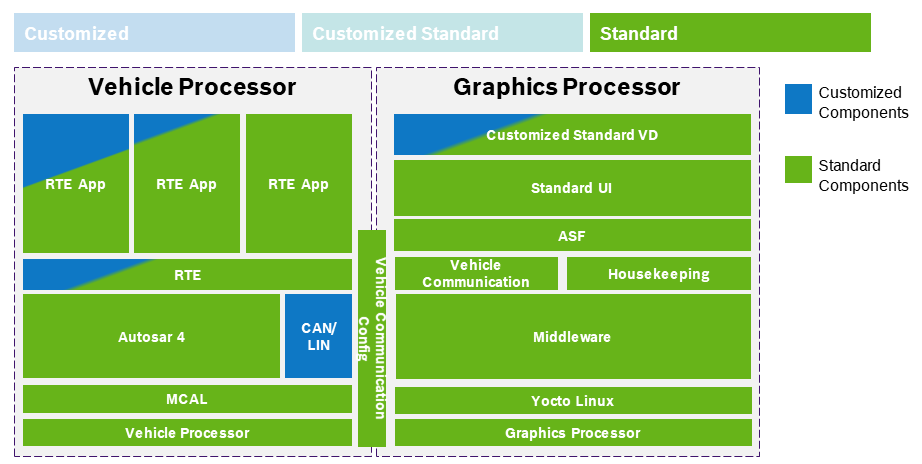
\includegraphics[width=\textwidth]{img/2_stand_der_technik/STICC_3_neu}
	\caption[Architektur der Standard-Ausbaustufe]{Architektur der Standard-Ausbaustufe \cite{bosch}}
	\label{fig:standard}
\end{figure}

Die Customized-Standard-Ausbaustufe bietet etwas mehr Auswahlmöglichkeiten für den Kunden. Trotzdem sehen sich die Endergebnisse sehr ähnlich, wie Abbildung \ref{fig:cu_st} zeigt, ist der Blauanteil etwas größer. Dadurch ergibt sich für den Kunden eine etwas größer Anpassungsmöglichkeit. So kann er in dieser Ausbaustufe das Visual Design komplett anpassen und zum Teil auch die Standard UI. \\

\begin{figure}[htb]
	\centering
	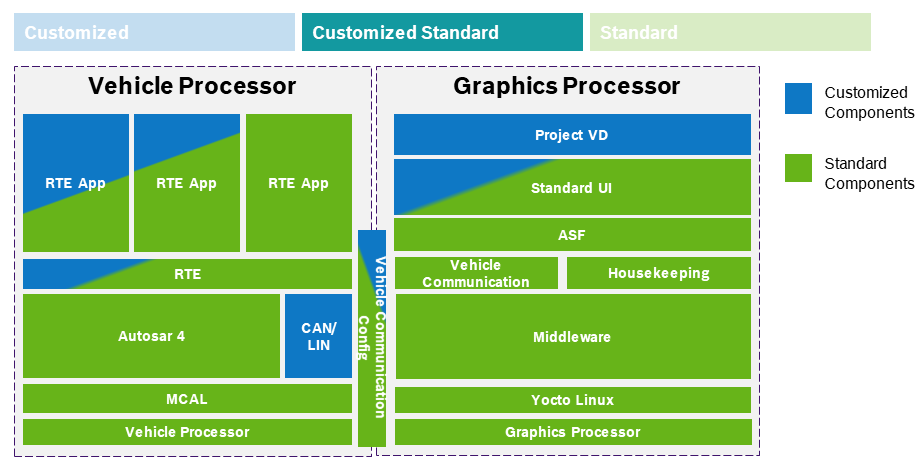
\includegraphics[width=\textwidth]{img/2_stand_der_technik/STICC_2_neu}
	\caption[Architektur der Customized-Standard-Ausbaustufe]{Architektur der Customized-Standard-Ausbaustufe \cite{bosch}}
		\label{fig:cu_st}
	\end{figure}
	 
Die letzte Ausbaustufe, in Abbildung \ref{fig:customized} zu sehen, bietet für den Kunden die größtmögliche Anpassungsmöglichkeit. Die Customized-Ausbaustufe ist bezüglich der Entwicklung - und damit auch der Kosten - die aufwendigste Stufe. Diese Stufe wird vor allem von den großen Herstellern gewählt. Zum einen um sich von den Wettbewerbern abzuheben und zum anderen, weil durch die Skaleneffekte der Kostenanteil beim Einzelfahrzeug geringer ausfällt.

\begin{figure}[htb]
	\centering
	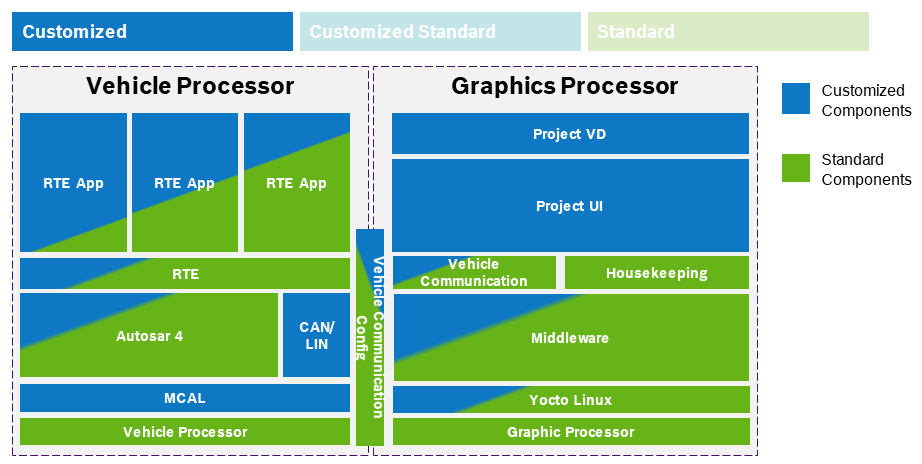
\includegraphics[width=\textwidth]{img/2_stand_der_technik/STICC_1_neu}
	\caption[Architektur der Customized-Ausbaustufe]{Architektur der Customized-Ausbaustufe \cite{bosch}}
	\label{fig:customized}
\end{figure}

Die bisherigen Nachteile der aktuellen Umsetzung sind zum einen die Hochlaufzeit und zum anderen die eingeschränkten Anpassungsmöglichkeiten.\\

\subsection{CGI Studio}
Die \ac{HMI}-Entwicklung erfolgt mit CGI Studio. CGI Studio ist das aktuelle Standardtool innerhalb der \ac{BEG}.\\

\glqq CGI Studio ist eine skalierbare und hardwareunabhängige Softwareplattform. Die offene Architektur ermöglicht eine tiefe Integration und Automatisierung. Die Software erlaubt die Erstellung von brillanten und anpassbaren \acp{HMI} aller Art für den Automobilbereich und darüber hinaus.\grqq{} \cite{canderaFAQ}\\

CGI Studio wird von dem österreichischen Unternehmen SocioNext entwickelt. Das Tool funktioniert nach dem \ac{WYSIWYG}-Prinzip. Die Grafiken werden importiert und können dann in den Editor gezogen werden.\\

% Was ist MVC
% Model, View, Controller erklären & was von CGI wo dazu gehört
% Bisschen zur Umsetzung
\subsection{Model-View-Controller}
Der \ac{MVC} ist ein Entwurfsmuster, dass die Daten, die Handhabung der Daten und die Anzeige der Daten trennt. Das Model empfängt Nachrichten über \ac{CAN} vom \ac{KSS} und sendet Daten an den Controller oder die View. Die empfangenen Nachrichten sind entweder Daten des Fahrzeugs oder eine Kontrollanweisung. Daten können zum Beispiel, Geschwindigkeit, Temperatur oder Drehzahl, sein und werden direkt an den Viewcontroller innerhalb der View geschickt. Eine Kontrollanweisung könnte ein Tastendruck oder das Drehen eines Drehencoders sein. Zwischen Model und Viewcontrollern existiert noch ein Zustandsautomat der regelt welcher Screen wann angezeigt wird. Der Controller entscheidet, was angezeigt wird und die View entscheidet, wie etwas angezeigt wird.\\

\begin{figure}[htb]
	\centering
	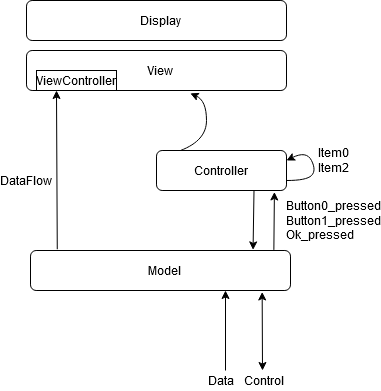
\includegraphics[width=10cm]{img/2_stand_der_technik/ModelViewControler}
	\caption{\acs{UML}-Diagramm eines Model-View-Controllers}
	\label{fig:mvc}
\end{figure}

\newpage

\subsubsection{Model}

% Quellen
% https://inside-docupedia.bosch.com/confluence/display/hmicore/Courier-based+HMI+Architecture

Die Model Komponente kümmert sich um das Empfangen und Weiterleiten von Nachrichten. Nachrichten, welche von dem \ac{KSS} kommen, müssen an die richtigen Empfänger verteilt werden. Ein Knopfdruck beispielsweise muss an den Controller geleitet werden um einen neuen Screen darzustellen. Eine Änderung der Geschwindigkeit muss jedoch an die View geschickt werden, damit der neue Wert in der Szene angezeigt wird.\\

Das Model stellt die, für die \ac{HMI}, relevanten Daten bereit. Das Model aktualisiert dann den Controller und die View mit Hilfe des Beobachtermusters. Das Model besitzt keine Abhängigkeiten gegenüber der Plattform. Im Model werden die Daten auf Plausibilität geprüft und wenn nötig in eine andere Einheit umgerechnet. Anschließend werden die Daten der View oder dem Controller zur Verfügung gestellt.\\

In CGI Studio wird das Model durch weitere Komponenten dargestellt, die sich um die korrekte Verteilung kümmern (z.B. Courier-Klasse). Diese sind im Folgenden nicht relevant und werden entsprechend nicht näher beschrieben.\\

\subsubsection{View}

Die View stellt die Daten aus dem Model grafisch dar. Die einzelnen Instrumente sind in Szenen aufgeteilt. Eine Szene kann zum Beispiel die Drehzahlanzeige oder die Außentemperaturanzeige sein. Die einzelnen Szenen werden im Scene Composer von CGI Studio erstellt. Die View fasst alle Szenen (Viewcontroller) zusammen, wie in Abbildung \ref{fig:scene} dargestellt. Für jede Szene existiert ein eigener Viewcontroller. Jeder Viewcontroller kann die Eigenschaften der zugehörigen Szene verändern. Aus den verschiedenen Szenen wird ein Screen erstellt. Der Screen wird dann auf dem Display gerendert dargestellt.\\

\begin{figure}[htb]
	\centering
	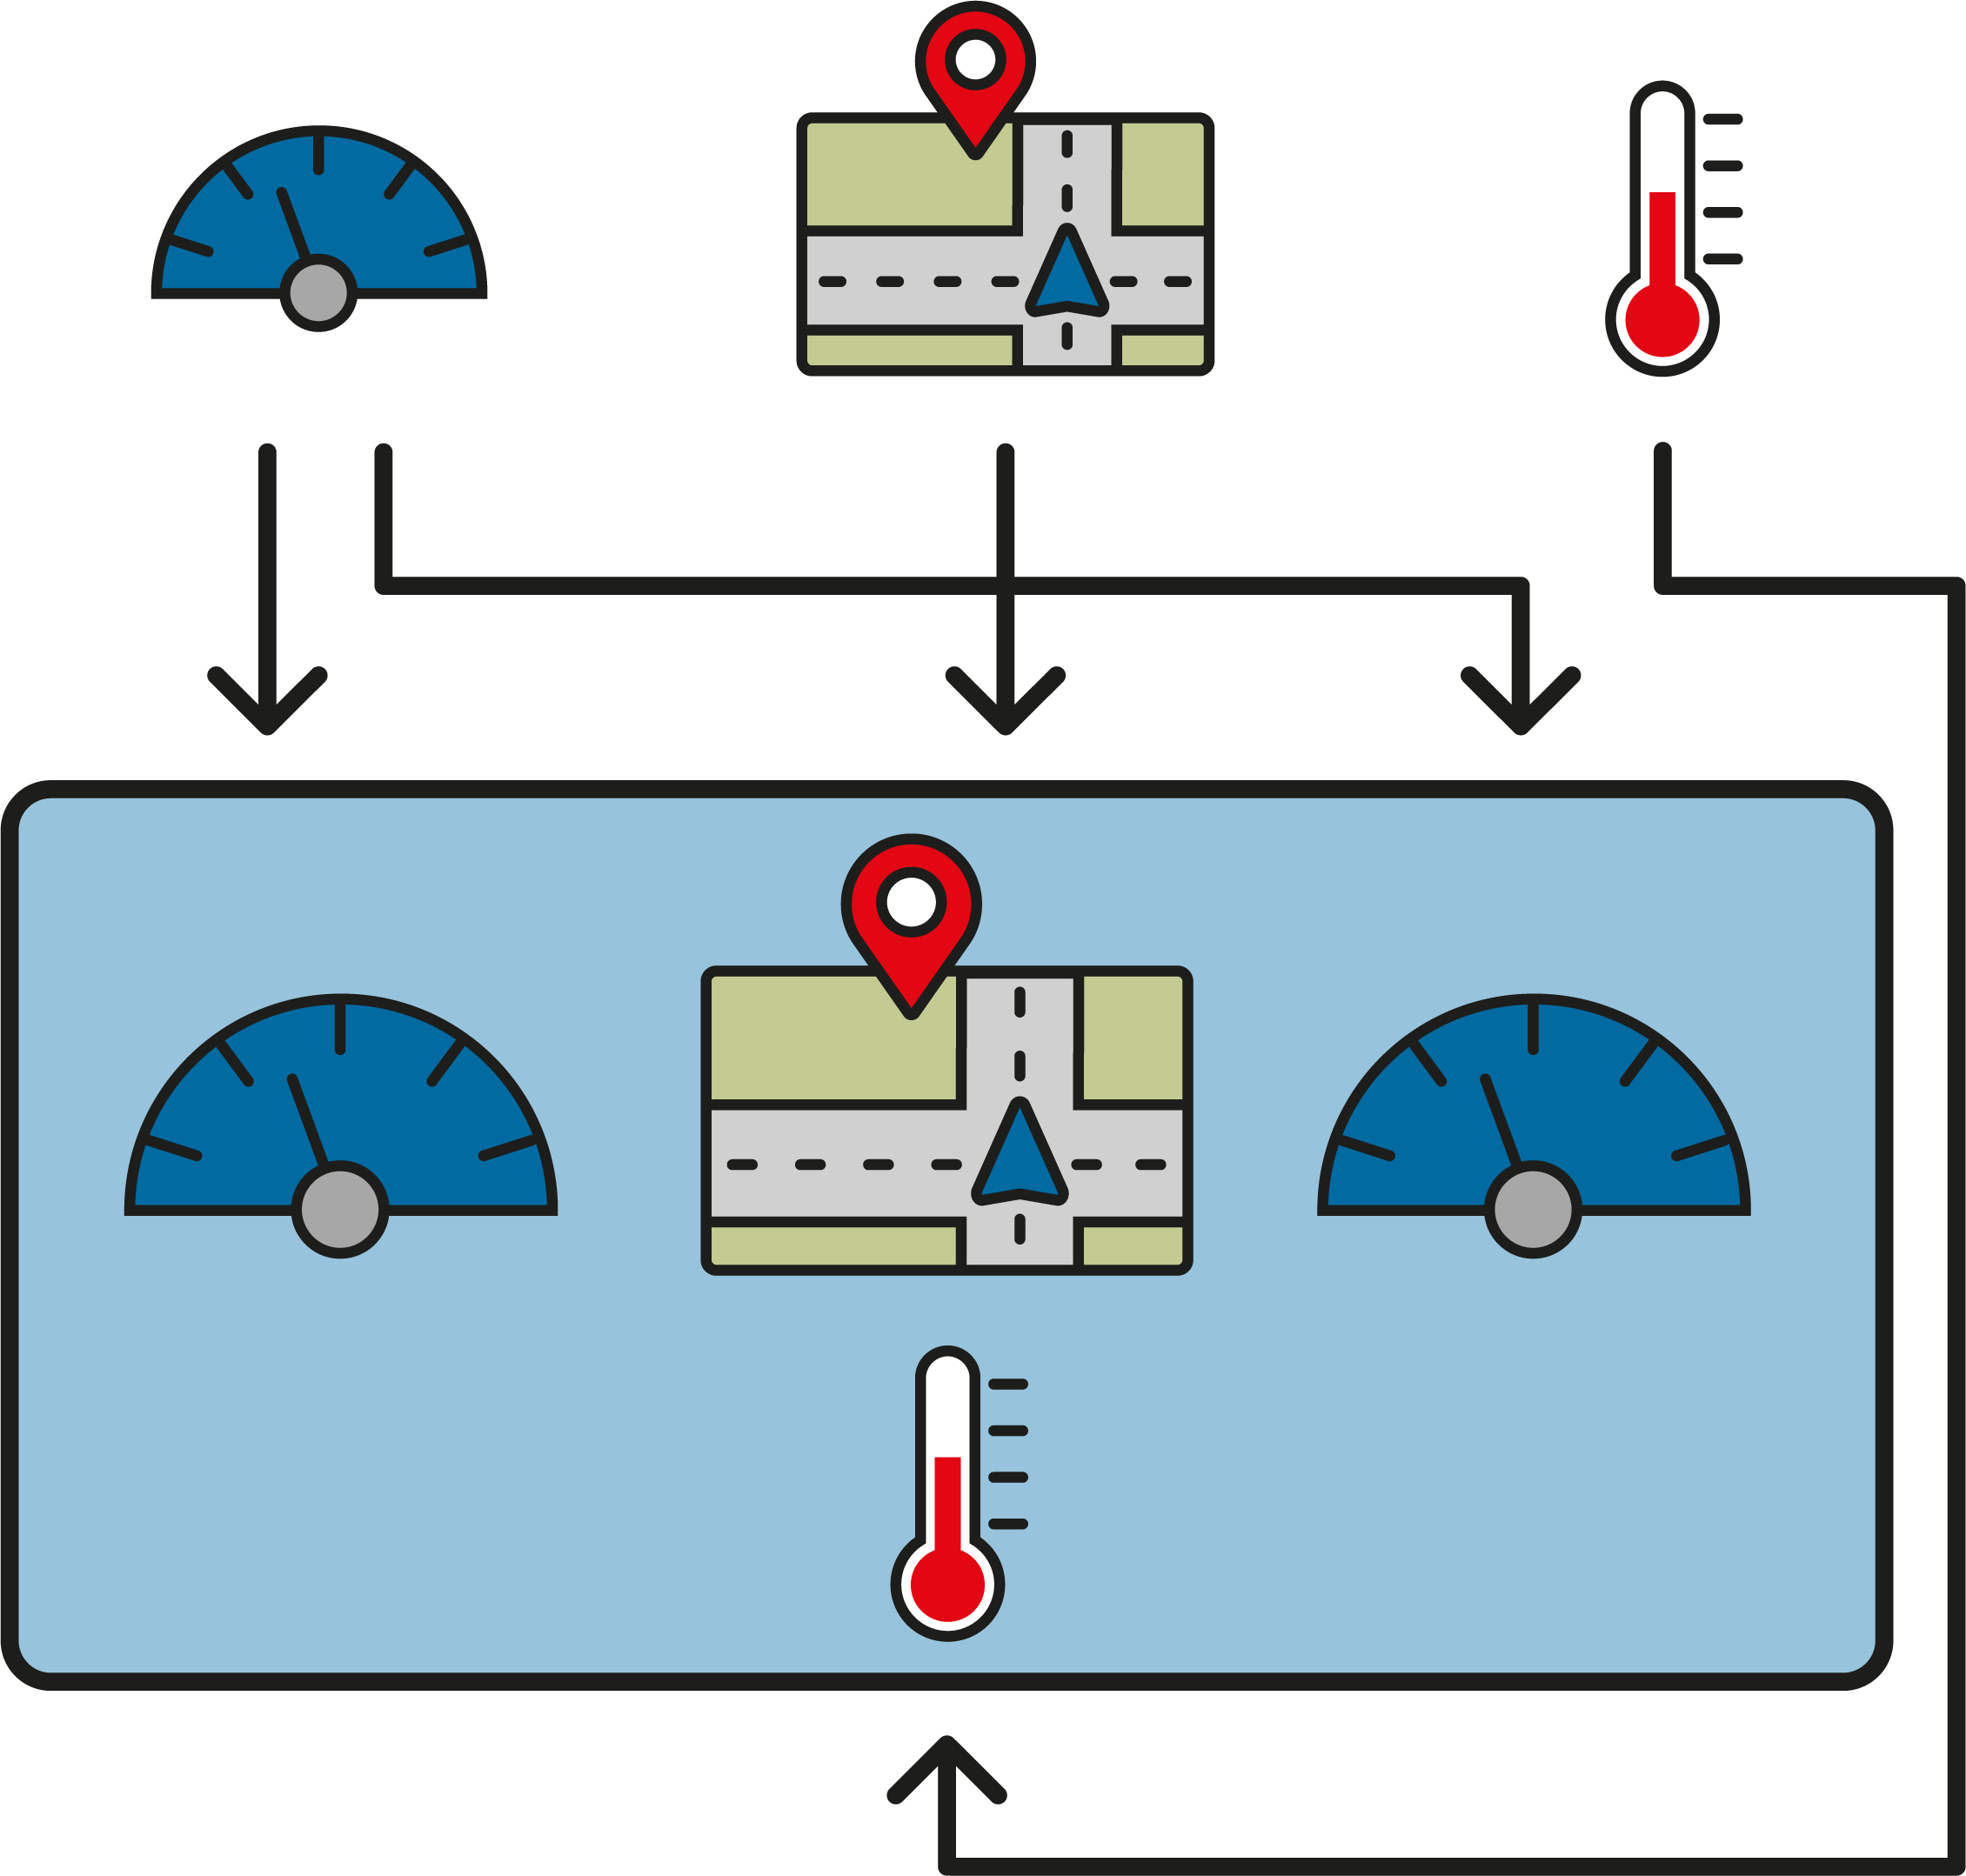
\includegraphics[width=14cm]{img/2_stand_der_technik/scene}
	\caption{Grafisches Beispiel einzelner Szenen zusammengesetzt zu einem Screen}
	\label{fig:scene}
\end{figure}




\subsubsection{Controller}
Der Controller reagiert auf Benutzerinteraktionen sowie Systemnachrichten und verändert basierend darauf die Anzeige des Kombiinstruments. Ein Controller besteht aus einem Zustandsautomaten. Jeder Zustand repräsentiert dabei eine definierte Anzeige auf dem Display. Durch einen Tastendruck oder andere Interaktionen wird zwischen den verschiedenen Zuständen gewechselt. Muss der Controller warten bis die View die alten Daten verarbeitet hat, benötigt der Controller ebenfalls einen Wartezustand.\\

\begin{figure}[htb]
	\centering
	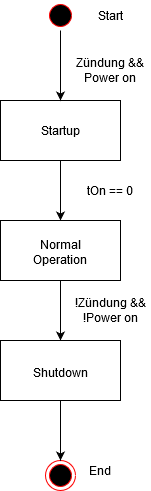
\includegraphics[width=4cm]{img/2_stand_der_technik/simple_statemachine}
	\caption{Beispielhafter Zustandsautomat eines Controllers}
	\label{fig:state}
\end{figure}

Abbildung \ref{fig:state} zeigt einen möglichen Zustandsautomat. Der abgebildete Zustandsautomat ist sehr simpel und enthält nur drei Zustände. Der erste Zustand \glqq Startup\grqq{} wird erreicht, wenn Klemme 15 geschlossen ist (Zündung an). Um hochzufahren benötigt das \ac{HMI} eine bestimmte Zeit, ist diese Zeit abgelaufen wechselt der Zustandsautomat in den \glqq Normal Operation\grqq{} Zustand. In diesem Zustand könnte zum Beispiel die aktuelle Geschwindigkeit und die Drehzahl des Motors angezeigt werden. Der Zustandsautomat verbleibt so lange in diesem Zustand bis Klemme 15 wieder geöffnet wird (Zündung aus). Durch diese Änderungen wechselt der Zustandsautomat in den \glqq Shutdown\grqq{} Zustand und beendet alle Funktionen.\\

Bisher wurden die Zustandsautomaten mit visualSTATE erstellt und dann dem Projekt hinzugefügt, mittlerweile bietet CGI Studio dafür eine eigene Lösung innerhalb des SceneComposer.\\
 

%bisschen mehr text
\subsection{Qualitätskriterien nach ISO 25010}\label{qualitaet}

Zu den Anforderungen werden in diesem Fall auch die Qualitätskriterien nach der ISO 25010 gezählt. Die ISO 250XX Reihe beschäftigt sich mit der Qualität und Bewertung von Software. Die ISO 25010 beschäftigt sich speziell mit dem Qualitätsmodell und passenden Leitlinien. Die ISO umfasst insgesamt 31 Qualitätskriterien, die sich auf acht übergeordnete Punkte verteilen. Eine Übersicht aus der ISO 25010 ist in Abbildung \ref{fig:Kriterien} dargestellt.\\

\begin{figure}[htb]
	\centering
	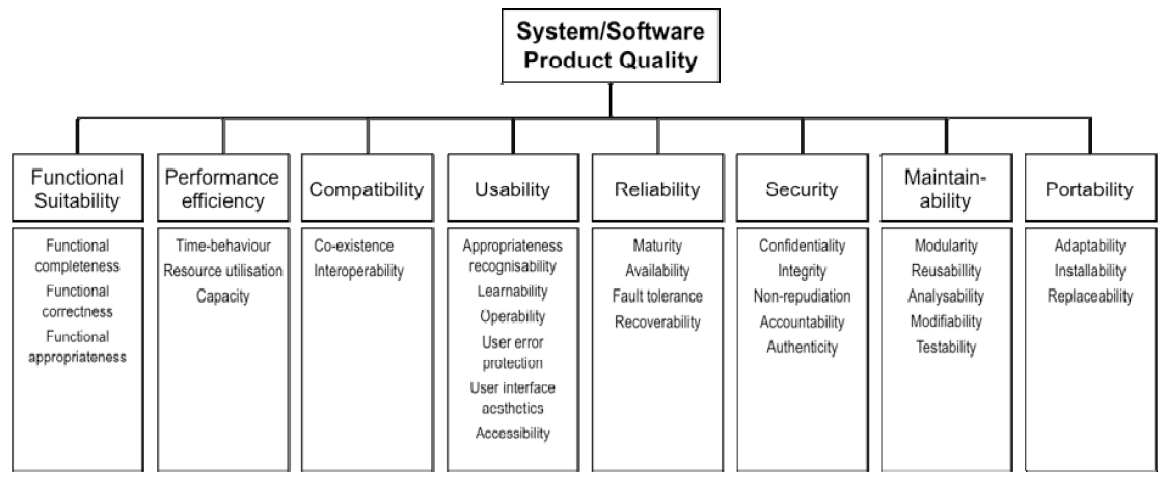
\includegraphics[width=\textwidth]{img/3_entwicklung_neues_kontept/Qualitaetskriterien}
	\caption[Qualitätskriterien aus der ISO 25010]{Qualitätskriterien aus der ISO 25010 \cite{iso25010}}
	\label{fig:Kriterien}
\end{figure}

Im Folgenden werden alle Qualitätskriterien kurz erläutert. \\
%Anschließend folgt eine Übersicht der Kriterien die im Hinblick auf das Architekturkonzept besonders relevant sind.\\

Die Functional Suitability beschreibt den Grad, in dem ein System Funktionen bietet, die den vorausgesetzten Bedürfnissen entsprechen. Dabei gibt die Functional completeness an wie weit die angegebenen Aufgaben und Benutzerziele durch den Funktionssatz abgedeckt werden. Im Gegensatz dazu zielt die Functional correctness darauf ab, in wie weit die richtigen Ergebnisse mit dem erforderlichen Grad an Präzision geliefert werden. Das letzte Kriterium die Functional appropriateness zeigt in wie weit Funktionen das Erfüllen bestimmter Aufgaben und Ziele erleichtert \cite{iso25010}.\\

Die Performance efficiency sagt etwas über die Performance relativ zu der Menge an Ressourcen unter gegebenen Bedingungen aus. Time-behaviour zielt dabei auf die Reaktions- und Bearbeitungszeit des Systems. Die Resource utilisation gibt die Anzahl und Arten der Ressourcen wieder (z.B. CPU, GPU, RAM, ROM). Die Capacity sagt aus, ob die Kapazität ausreicht (bsp. Anzahl an Menüs, Benutzter, usw.) \cite{iso25010}.\\

Die Compatiblity befasst sich mit dem Grad in dem ein System Informationen mit anderen Systemen austauschen kann, während sie die gleiche Hardware- oder Softwareumgebung teilen. Die Co-existence geht dabei darauf ein, in wie weit das Produkt die Ressourcen und Umgebung mit anderen Produkten teilen kann, ohne Performance zu verlieren. Bei der Interoperability wird beleuchtet, in wie fern zwei oder mehr Systeme Informationen austauschen und diese nutzen \cite{iso25010}.\\

Die Usability bezieht sich auf den Grad bis zu dem ein genutztes System, durch bestimmte Benutzter spezifizierte Ziele effektiv, effizient und zufriedenstellend erreicht. Dabei beschreibt die Appropriateness recognisability in wie weit der Nutzer erkennen kann, ob das System angemessen für seine Bedürfnisse ist, basierend auf den ersten Eindrücken und/oder mitgelieferten Dokumenten. Die Learnability zielt darauf ab wie einfach das Produkt oder System von bestimmten Nutzern erlernt werden kann um das Produkt oder System mit Wirksamkeit, Effizienz, Risikofreiheit und Zufriedenheit zu nutzen. Die Operability geht darauf ein, wie die Eigenschaften die Nutzung und Kontrolle vereinfachen. Die User error protection beschäftigt sich damit wie der Nutzer vor fehlerhaften Eingaben geschützt wird. Bei der User Interface aesthetics wird untersucht, ob die Interaktionen mit dem Benutzerinterface erfreulich und befriedigend sind. Die Accessibility analysiert, ob das Produkt von möglichst vielen Benutzern nutzbar ist \cite{iso25010}. \\


Die Reliability befasst sich damit, bis zu welchem Grad ein System, spezifizierte Funktionen unter bestimmten Bedingungen für eine definierten Zeitraum ausführt. Dabei beschäftigt sich die Maturity damit wie zuverlässig das Produkt bei normalem Betrieb ist. Die Availability beleuchtet, wie zugänglich das Produkt bei Bedarf ist und wie lange das Produkt ohne Fehler funktioniert. Die Fault tolerance überprüft, ob das System wie beabsichtigt funktioniert, trotz Hardware- oder Softwarefehler. Die Recoverability zielt darauf ab, ob das Produkt oder System im Falle einer Unterbrechung oder eines Ausfalls, die Daten die betroffen sind direkt wiederherstellen und den gewünschten Zustand des Systems wiederherstellen kann \cite{iso25010}.\\


Die Security interpretiert den Grad in dem ein System Informationen und Daten vor unberechtigten Zugriffen schützt. Die Confidentiality überprüft dabei, ob das System sicherstellt, dass nur autorisierte Benutzer Zugriff auf Daten bekommen. Die Integrity beschäftigt sich damit, ob das System unautorisierten Zugriff auf, oder Modifikation im Programm oder Daten verhindert. Non-repudiation erörtert wie verschiedene Aktionen nachgewiesen werden können. Die Accountability dagegen beschäftigt sich damit wie weit Handlungen eines Benutzers nachweisbar sind. Die Authenticity zielt darauf ab, ob die Identität einer Ressource nachgewiesen werden kann \cite{iso25010}\\


Maintainability gibt den Grad der Effektivität und Effizienz mit der ein System modifiziert werden kann an. Die Modularity beleuchtet, ob das Produkt in einzelne unabhängige Komponenten zerlegt und wie die einzelnen Komponenten zusammengefügt werden können. Die Reusability beschäftigt sich damit, wie weit ein Asset wiederverwendbar oder für andere Assets benutzbar ist. Die Analysability legt dar, wie effektiv und effizient beurteilt werden kann wie sehr andere Teile von einer beabsichtigten Änderung betroffen sind. Die Modifiability prüft, wie effektiv und effizient ein Produkt geändert werden kann ohne Auftreten von Mängeln, oder eine Verschlechterung der Produktqualität. Die Testability beschreibt, wie effektiv und effizient Testkriterien, für ein System, eingeführt und getestet werden können \cite{iso25010}.\\


Die Portability legt den Grad der Effektivität und Effizienz mit der ein System von einer Hard- oder Softwareumgebung in eine andere transferiert werden kann fest. Die Adaptability zielt darauf ab, ob sich ein System effektiv und effizient auf verändernde Hardware und Software anpasst. Die Installability beschäftigt sich damit, wie effektiv und effizient sich ein Produkt in einer speziellen Umgebung installieren und deinstallieren lässt. Die Replaceability legt dar, wie das System ein anderes System für den gleichen Zweck in der gleichen Umgebung ersetzt \cite{iso25010}.\\


%aus dem Buch Entwurfsmuster 
\subsection{Entwurfsmuster}
Bei der Entwicklung der Architektur soll auf Entwurfsmuster zurückgegriffen werden. Entwurfsmuster im Bereich Softwareentwicklung wurden maßgeblich von der \ac{GoF} etabliert. Die Gang of Four besteht aus den Softwareexperten Erich Gamma, Richard Helm, Ralph Johnson und John Vlissides, zusammen brachten sie 1994 das Buch Entwurfsmuster heraus.\\

Im Buch werden 23 verschieden Entwurfsmuster eingeführt und ausführlich erklärt. Entwurfsmuster sollen dabei helfen, objektorientierten Code wiederverwendbarer zu gestalten. Die \ac{GoF} versucht immer wiederkehrende Entwurfsprobleme zu identifizieren und eine allgemeingültige Lösung dafür anzubieten. Die Entwurfsmuster wurden dabei in drei übergeordnete Kategorien eingeteilt, Erzeugungsmuster, Strukturmuster und Verhaltensmuster. Die Muster wurden zusätzlich noch eingeteilt in klassenbasiert oder objektbasiert. Daraus entsteht die Matrix aus Tabelle \ref{tab:pattern}.\\

\begin{table}[h]
	\centering
	\caption[Übersicht der Entwurfsmuster aus dem Buch Entwurfsmuster]{Übersicht der Entwurfsmuster aus dem Buch Entwurfsmuster \cite{noauthor2011EntwurfsmusterElemente} }
	\label{tab:pattern}
	\begin{tabular}{|c|c|c|c|}\cline{2-4}
		\multicolumn{1}{c|}{} 			& Erzeugungsmuster  & Strukturmuster 	& Verhaltensmuster	 \\ \hline
		\multirow{2}{*}{klassenbasiert} & Fabrikmethode  	&  Adapter 			& Interpreter		 \\
		 								&				 	&					& Schablonenmethode	 \\ \hline
		\multirow{9}{*}{objektbasiert} 	& Abstrakte Fabrik  & Adapter  			& Befehl			 \\
										& Erbauer			& Brücke			& Beobachter		 \\
										& Prototyp			& Dekorierer		& Besucher			 \\
										& Singelton			& Fassade			& Iterator			 \\
										&					& Fliegengewicht	& Memento			 \\
										&					& Kompositum		& Strategie			 \\
										&					& Proxy				& Vermittler		 \\
										&					&					& Zustand			 \\
										&					&					& Zuständigkeitskette\\ \hline
	\end{tabular} 
	
\end{table} 

Erzeugungsmuster beschäftigen sich mit der Erzeugung von Objekten. Strukturmuster beschäftigen sich mit der Zusammensetzung von Klassen. Verhaltensmuster beschäftigen sich damit wie Klassen und Objekte miteinander arbeiten. Die zweite Einteilung, bestimmt, ob das Muster sich auf Klassen oder Objekte bezieht \cite{noauthor2011EntwurfsmusterElemente}. \\

Die oben genannten Entwurfsmuster wurden 1994 veröffentlicht gehören heute aber immer noch zum Standard. Die Entwurfsmuster im Buch zielen größtenteils auf die Programmiersprache C++ ab, mittlerweile gibt es von anderen Softwareentwicklern eigens entwickelte Entwurfsmuster für andere Sprachen.\\

\subsection{Anforderungen an das HMI-Framework}
\label{use_cases}
%Use Cases
Das richtige Framework wird auf Basis von Use Cases ausgewählt. Diese Use Cases wurden 2017 für die Evaluation von \ac{CM} entwickelt und basieren auf den Funktionen von CGI Studio. Mit Hilfe der Use Cases soll festgestellt werden, ob ein \ac{HMI}-Framework, in Projekten, häufig benötigte Funktionen umsetzten kann.\\ 

Die Use Cases gliedern sich in sechs Kategorien. Innerhalb der Kategorien gibt es obligatorische und optionale Anforderungen. In den nachfolgenden Kapitel wird auf diese Kategorien näher eingegangen.\\

\begin{itemize}
	\item Cluster \ac{HMI}
	\item Visual Appearance
	\item Text- und Listenverhalten
	\item Externe Daten
	\item Überlappung
	\item Komplexes Listenverhalten
\end{itemize}

\subsubsection{Cluster HMI} 
%In der Kategorie Cluster \ac{HMI} liegt der Fokus auf den Grundfunktionen von Instrument Clustern. Dazu zählen Nadelinstrumente und Warnlampen. 

%In dieser Kategorie müssen mindestens zwei Nadelinstrumente umgesetzt werden. Die Nadeln jedes Instruments müssen jeweils von einem eigenen Eingangssignal ansteuerbar sein. Die Nadeln müssen über einen Nachleuchten-Effekt verfügen. Die Geschwindigkeit und Drehzahl müssen textbasiert angezeigt werden und die Einheit von \si[per-mode=repeated-symbol]{\kilo\meter\per\hour} in \si[per-mode=repeated-symbol]{mi\per\hour} änderbar sein. Ebenfalls muss ein Warnlampenset implementierbar sein, zu Warnlampen gehören unter anderem das Anschnall-Symbol oder die Motor-Kontrollleuchte. Die Symbole dafür sind nach ISO 2575:2010 standardisiert.\\

%neu
In der Kategorie Cluster HMI sollen die Standardfunktionen von Instrument Clustern überprüft werden. Es handelt sich dabei um Nadelinstrumente und Warnlampen.\\

Die Nadel des Nadelinstruments muss sich abhängig vom Eingangssignal bewegen. Sie soll einen Nachleuchten-Effekt besitzen, wenn sie sich bewegt. Neben der analogen Anzeige soll auch eine digitale Anzeige der Werte möglich sein. Eine textbasierte Einheitenanzeige muss umschaltbar zwischen Kilometer und Meile sein.\\

Zudem muss ein Warnlampenset implementierbar sein, zu Warnlampen gehören unter anderem das Anschnall-Symbol oder die Motor-Kontrollleuchte. Die Symbole dafür sind nach ISO 2575:2010 standardisiert.\\

%bild davon

\subsubsection{Visual Appearance}
\label{visual}
%neu
In dieser Kategorie sollen verschiedene visuelle Effekte überprüft werden. Dazu gehört zum Beispiel die Darstellung der \ac{ACC}-Funktion mit einem 3D-Modell eines Fahrzeugs.\\

Die \ac{ACC}-Funktion regelt den Abstand zum vorausfahrenden Fahrzeug über die Geschwindigkeit. Dadurch bremst und beschleunigt das Fahrzeug von selbst.\\

Ein 3D-Modell eines Fahrzeugs soll sich analog zum aktuellen Zustand entweder zum Betrachter hinbewegen oder wegbewegen. Das 3D-Modell stellt das vorfahrende Fahrzeug dar. Erhöht sich die Geschwindigkeit, muss der Abstand größer werden, da sich der Bremsweg vergrößert. Umgekehrt kann der Abstand kleiner werden, wenn sich die Geschwindigkeit verringert.\\

Neben dem 3D-Modell soll mit Zahlen der aktuell gehaltene Abstand in Metern und Sekunden angezeigt werden.\\

Außerdem soll es möglich sein, die Außenfarbe des Fahrzeugs, abhängig von einem Eingangssignal, zu ändern.\\


\subsubsection{Text- und Listenverhalten}
In dieser Kategorie müssen verschiedene Listen implementierbar sein, z.B. vordefinierte Listen mit ca. 20 Einträgen und lange Listen mit ca. 500 Einträgen. Die Listen müssen scrollbar sein. Zum einen muss von Eintrag zu Eintrag gescrollt werden können und zum anderen zehn Einträge auf einmal gescrollt werden können.\\

Von einer Liste soll in eine andere Liste gewechselt werden können und alle Texte müssen übersetzbar sein. Sprachen müssen anlegbar sein, bei einem Wechsel der Sprache müssen alle Texte übersetzt werden.

\subsubsection{Externe Daten}
Ein Video aus einer externen Videoquelle muss abspielbar sein

\subsubsection{Überlappung}
Mit einem eingehenden Anruf-Fenster muss die Möglichkeit zur Überlappung demonstriert werden. Das überlappende Fenster muss transparent sein, damit der Hintergrund sichtbar bleibt. Die im Hintergrund verbliebenen Instrumente sollen weiterhin aktualisiert werden.

\subsubsection{Komplexes Listenverhalten}
Hier soll eine Medienliste mit ca. 10000 Einträgen implementiert werden. Die Form der Liste muss eine Kurve sein. Die Größe der Elemente soll von der Position abhängig sein, in der Mitte das Größte nach außen hin werden die Elemente kleiner. Abhängig von der Länge der Texteinträge sollen die Listeneinträge unterschiedliche Größen und Formen haben. Das Scrollverhalten muss ein Pixel zu Pixel scrollen ermöglichen. Die Liste soll beim Stoppen des Scrollens einrasten, dabei sollen keine halben Elemente zu sehen sein. Jeder Eintrag besteht aus einem Text, Bild und Button. Jeder Eintrag soll einen Fortschrittsbalken haben der kontinuierlich aktualisiert wird. Am Ende der Liste muss eine Abprallen-Animation stattfinden.

